% my memo
%   make hldd
%   cp design.pdf gsa/
%
%\documentstyle[a4]{article} 

%\documentclass[a4paper]{article}
\documentclass[12pt,a4paper]{article}

% same w/ Doxygen
%\documentclass[a4paper]{book}
\usepackage{a4wide}
\usepackage{makeidx}
\usepackage{fancyhdr}
%\usepackage{graphicx}
\usepackage{multicol}
\usepackage{float}
\usepackage{textcomp}
\usepackage{alltt}
\usepackage{times}
\usepackage[utf8]{inputenc}

% Ubuntu texlive-latex-recommended package
% /usr/share/texmf-texlive/tex/latex/listings
\usepackage{listings}

%%\usepackage{apidoc_latex/doxygen}
%\NeedsTeXFormat{LaTeX2e}
%\ProvidesPackage{doxygen}
%\RequirePackage{calc}
%\RequirePackage{array}
%\pagestyle{fancyplain}
%\newcommand{\clearemptydoublepage}{\newpage{\pagestyle{empty}\cleardoublepage}}
%\renewcommand{\chaptermark}[1]{\markboth{#1}{}}
%\renewcommand{\sectionmark}[1]{\markright{\thesection\ #1}}
%
%\lhead[\fancyplain{}{\bfseries\thepage}]
%        {\fancyplain{}{\bfseries\rightmark}}
%\rhead[\fancyplain{}{\bfseries\leftmark}]
%        {\fancyplain{}{\bfseries\thepage}}
%\rfoot[\fancyplain{}{\bfseries\scriptsize OpenPTS v0.0.1 }]{}
%\lfoot[]{\fancyplain{}{\bfseries\scriptsize OpenPTS v0.0.1 }}
%\cfoot{}

%\makeindex
\setcounter{tocdepth}{3}
\renewcommand{\footrulewidth}{0.4pt}


\usepackage[dvipdfm]{graphicx, color}
%\usepackage{mediabb}

% Ubuntu - ebb - texlive-base-bin
% Fedora12 - Error
%   $ ebb bios_pcr0.png
%   Can't handle file type for file named bios_pcr0.png
%   >>> use ebbx :-(
%
% version :  ebb, version Version 0.5.2, Copyright (C) 1998, 1999 by Mark A. Wicks
% $ rpm -qf /usr/bin/ebb
% dvipdfm-0.13.2d-41.fc12.x86_64
%

% Fedora12 - fig not imported. the error is:
%Conversion via ->zcat -f ./grub_pcr4.png | gs -q -sPAPERSIZE=a0 -sDEVICE=pdfwrite -dCompatibilityLevel=1.2 -dUseFlateCompression=true -dSAFER -sOutputFile=/tmp/dvipdfm.EBY2D0 - -c quit<- failed
%)
%pdf: image inclusion failed for (grub_pcr4.png).
%Image special ignored.
%][40(./grub_pcr5.png<?>Error: /syntaxerror in (binary token, type=137)
%Operand stack:
%
%Execution stack:
%   %interp_exit   .runexec2   --nostringval--   --nostringval--   --nostringval--   2   %stopped_push   --nostringval--   --nostringval--   --nostringval--   %false   1   %stopped_push   1878   1   3   %oparray_pop   1877   1   3   %oparray_pop   1861   1   3   %oparray_pop   1755   1   3   %oparray_pop   --%nostringval--   %errorexec_pop   .runexec2   --nostringval--   --nostringval--   --nostringval--   2   %stopped_push
%Dictionary stack:
%   --dict:1158/1684(ro)(G)--   --dict:0/20(G)--   --dict:70/200(L)--
%Current allocation mode is local




\usepackage{url}
% http://en.wikibooks.org/wiki/LaTeX/Hyperlinks
%\usepackage{hyperref}

%\addtolength{\oddsidemargin}{-.875in}
%\addtolength{\evensidemargin}{-.875in}
%\addtolength{\textwidth}{1.75in}

%\addtolength{\topmargin}{-.875in}
%\addtolength{\textheight}{1.75in}


%\title{Open Platform Trust Services - Architecture and Design}
%\author{Seiji Munetoh}  
%\date{May 10, 2010} 

\begin{document} 

%\maketitle  
%\clearpage 
\begin{titlepage}
\vspace*{7cm}
\begin{center}
{\Large Open Platform Trust Services - Architecture and Design \\[1ex]\large Version 0.2.0 }\\
\vspace*{1cm}
{\large Seiji Munetoh}\\
\vspace*{0.5cm}
%{\small May 11, 2010}\\
{\small \today}\\

\end{center}
\end{titlepage}


%\clearemptydoublepage
\pagenumbering{roman}


\tableofcontents

\clearpage 
%\clearemptydoublepage
\pagenumbering{arabic}

%%%%%%%%%%%%%%%%%%%%%%%%%%%%%%%%%%%%%%%%%%%%%%%%%%%%%%%%%%%%%%%%%%%%%%%%%%%%%%
%%%%%%%%%%%%%%%%%%%%%%%%%%%%%%%%%%%%%%%%%%%%%%%%%%%%%%%%%%%%%%%%%%%%%%%%%%%%%%
\section{Introduction} 
%%%%%%%%%%%%%%%%%%%%%%%%%%%%%%%%%%%%%%%%%%%%%%%%%%%%%%%%%%%%%%%%%%%%%%%%%%%%%%
%%%%%%%%%%%%%%%%%%%%%%%%%%%%%%%%%%%%%%%%%%%%%%%%%%%%%%%%%%%%%%%%%%%%%%%%%%%%%%

\subsection{Purpose} 

The purpose of this design document is to provide a description of
the design of Open Platform Trust Services (OpenPTS).

\subsection{Scope} 

This document is the Architectural Design Document prepared for OpenPTS.

\subsection{Overview}

Section 1 is this introduction.
System Overview and Architecture is described in section 2 and 3.


\subsection{References} 

{\bf TCG Standards}

OpenPTS supports 

TCG XML Schemas, 

\begin{itemize}
\item Infrastructure Work Group Core Integrity Schema Specification, Version 1.0.1\cite{core_integrity_schema}
\item Infrastructure Work Group Simple Object Schema Specification, Version 1.0\cite{simple_object_schema}
\item Infrastructure Work Group Reference Manifest (RM) Schema Specification, Version 1.0\cite{rm_schema}
\item Infrastructure Work Group Integrity Report Schema Specification, Version 1.0\cite{integrity_report_schema}
\item Infrastructure Work Group Verification Result Schema Specification, Version 1.0\cite{verification_result_schema}
\item Infrastructure Work Group Security Qualities Schema Specification Version 1.1, Revision 7.0\cite{qualities_schema}
\end{itemize}

and APIs, 

\begin{itemize}
\item TNC IF-IMC Specification, Version 1.2\cite{ifimc}
\item TNC IF-IMV Specification, Version 1.2, Revision 8\cite{ifimv}
\end{itemize}

and protocol

\begin{itemize}
\item TNC IF-M: TLV Binding Version 1.0, Revision 37\cite{ifmtlv}
\item TF-M(PTS)\cite{ifmpts}
\end{itemize}


{\bf Open Source Components}

\begin{itemize}
\item ibmswtpm (IBM) \url{http://ibmswtpm.sourceforge.net/}
\item tboot (Intel) \url{http://sourceforge.net/projects/tboot}
\item tpm-dd (IBM) \url{http://tpmdd.sourceforge.net/}
\item TrouSerS (IBM) \url{http://trousers.sourceforge.net/}
\item Linux-IMA (IBM) \url{http://linux-ima.sourceforge.net/} 
\item OpenPTS (IBM) \url{http://openpts.sourceforge.jp/}
\item libtnc \url{http://sourceforge.net/projects/libtnc/}
\item TNC@FHH \url{http://trust.inform.fh-hannover.de/joomla/index.php/projects/tncfhh}
\end{itemize}


\subsection{Constraints}

At this time TPM v1.2 supports SHA1 only.
and all PC BIOS is based on SHA1.
PTS can manage the hash agility but at this time we are using SHA1. 


\subsection{Definitions and Acronyms}

\begin{description}
 \item[IMC]  Integrity Measurement Collector
 \item[IMV]  Integrity Measurement Verifier
 \item[IML]  Integrity Measurement Log
 \item[IR]   Integrity Report
 \item[RIMM] Reference Integrity Measurement Manifest
 \item[RM]   Reference Manifest
 \item[PTS]  Platform Trust Service
 \item[TCG]  Trusted Computing Group
 \item[TPM]  Trusted Platform Module
 \item[TNC]  Trusted Network Connect
\end{description}

\clearpage 


%%%%%%%%%%%%%%%%%%%%%%%%%%%%%%%%%%%%%%%%%%%%%%%%%%%%%%%%%%%%%%%%%%%%%%%%%%%%%%
%%%%%%%%%%%%%%%%%%%%%%%%%%%%%%%%%%%%%%%%%%%%%%%%%%%%%%%%%%%%%%%%%%%%%%%%%%%%%%
\section{System Overview}
%%%%%%%%%%%%%%%%%%%%%%%%%%%%%%%%%%%%%%%%%%%%%%%%%%%%%%%%%%%%%%%%%%%%%%%%%%%%%%
%%%%%%%%%%%%%%%%%%%%%%%%%%%%%%%%%%%%%%%%%%%%%%%%%%%%%%%%%%%%%%%%%%%%%%%%%%%%%%

PTS is defined by TCG to manage an integrity information.
Figure \ref{fig:tncarch} shows TNC architecture.
OpenPTS supports whole integrity management layer.
It provide IF-IMC and IF-IMV for TNC.
Collector and Verifier use IF-M protocol to attest the AR.

\begin{figure}[b!p]
  \begin{center}
    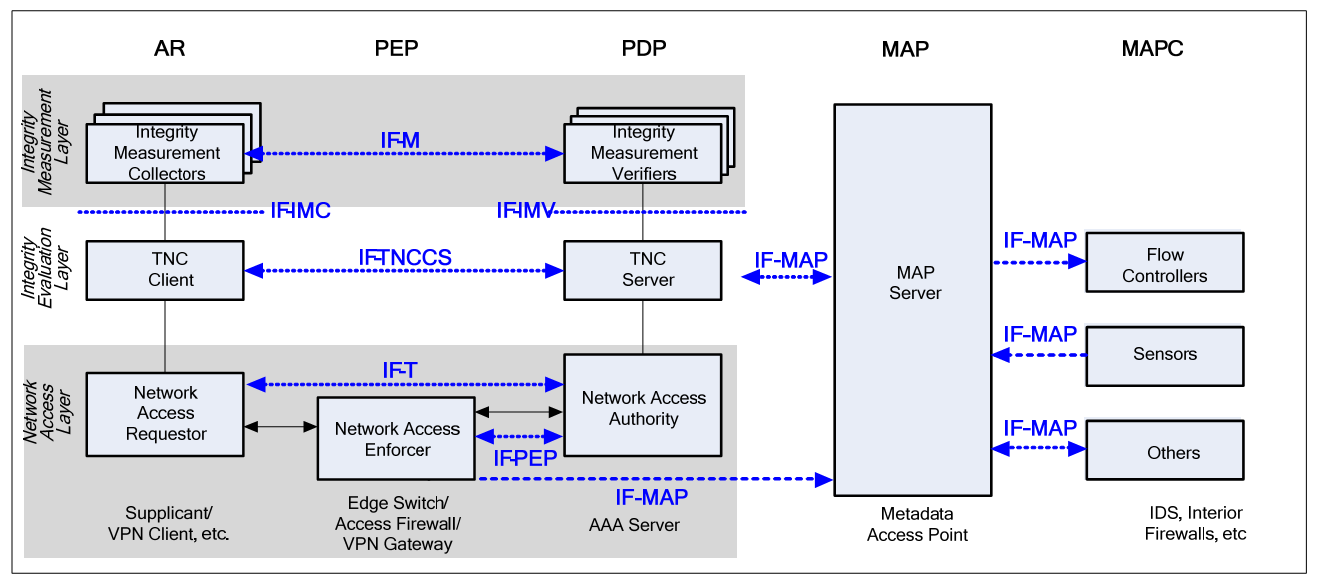
\includegraphics[width=15cm]{TNC_Architecture_1.png}
  \end{center}
  \caption{TNC Architecture\cite{tncarch}}
  \label{fig:tncarch}
\end{figure}


Figure \ref{fig:tncwpts} brakes down the Figure \ref{fig:tncarch} to internal component level.
OpenPTS integrates IMC and PTS thus IF-PTS API is not exposed.

\begin{figure}[b!p]
  \begin{center}
    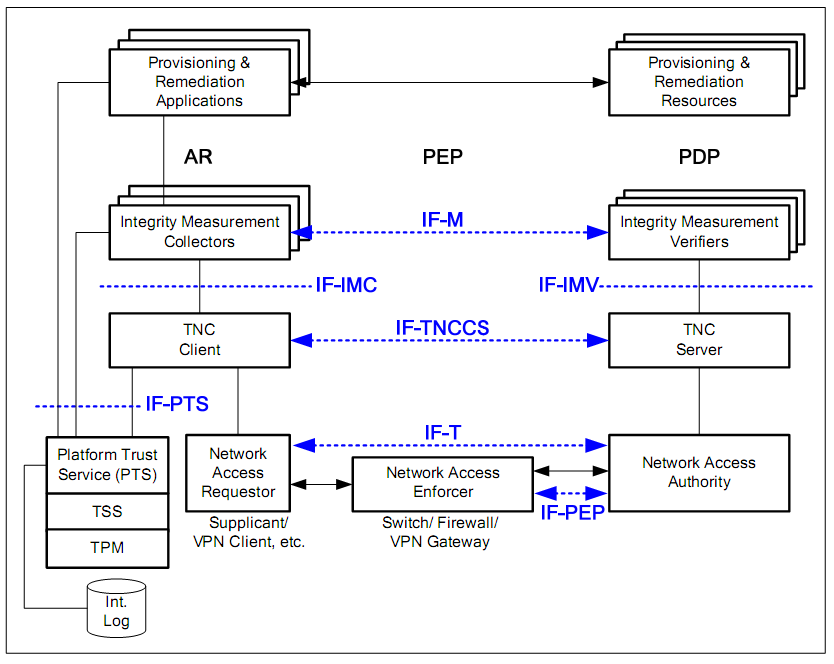
\includegraphics[width=12cm]{TNC_Architecture_2.png}
  \end{center}
  \caption{The TNC Architecture with the Trusted Platform Module (TPM)\cite{tncarch}}
  \label{fig:tncwpts}
\end{figure}


Figure \ref{fig:tncwimm} shows integrity management infrastructure.
OpenPTS supports XML schemas regrading this infrastructure which defined by TCG.

Unfortunately, there is no vendor who provide a Reference Manifest.
This OpenPTS provide an utility to create the manifest from existing integrity measurement log 


\begin{figure}[b!p]
  \begin{center}
    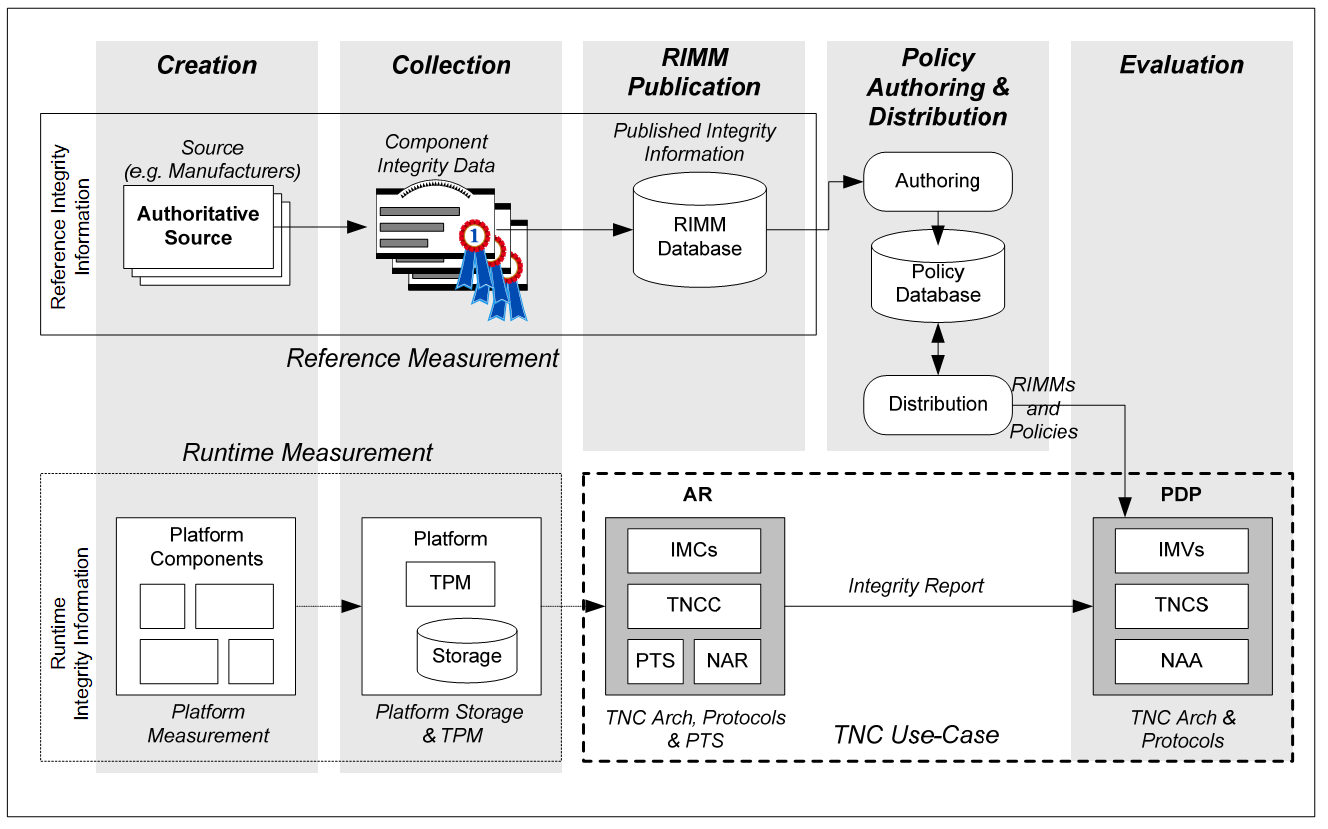
\includegraphics[width=15cm]{TNC_Architecture_3.png}
  \end{center}
  \caption{The TNC Architecture within the TCG Integrity Management Model\cite{tncarch}}
  \label{fig:tncwimm}
\end{figure}




\clearpage 

%%%%%%%%%%%%%%%%%%%%%%%%%%%%%%%%%%%%%%%%%%%%%%%%%%%%%%%%%%%%%%%%%%%%%%%%%%%%%%
%%%%%%%%%%%%%%%%%%%%%%%%%%%%%%%%%%%%%%%%%%%%%%%%%%%%%%%%%%%%%%%%%%%%%%%%%%%%%%
\section{System Architecture}
%%%%%%%%%%%%%%%%%%%%%%%%%%%%%%%%%%%%%%%%%%%%%%%%%%%%%%%%%%%%%%%%%%%%%%%%%%%%%%
%%%%%%%%%%%%%%%%%%%%%%%%%%%%%%%%%%%%%%%%%%%%%%%%%%%%%%%%%%%%%%%%%%%%%%%%%%%%%%

OpenPTS supports both TNC and standalone operations.

\subsection{TNC}

For TNC, OpenPTS is a library shared by TNC components.
Figure \ref{fig:openptstnc} shows block diagram of TNC with OpenPTS. 
Collector side, TNCC links libopenpts\_imc library. 
Verifier side, TNCS links libopenpts\_imv library. 
The IMC and IMV send and receive IF-M messages though TNC.
OpenPTS provide remote attestation capability for TNC.

\begin{figure}[b!p]
  \begin{center}
    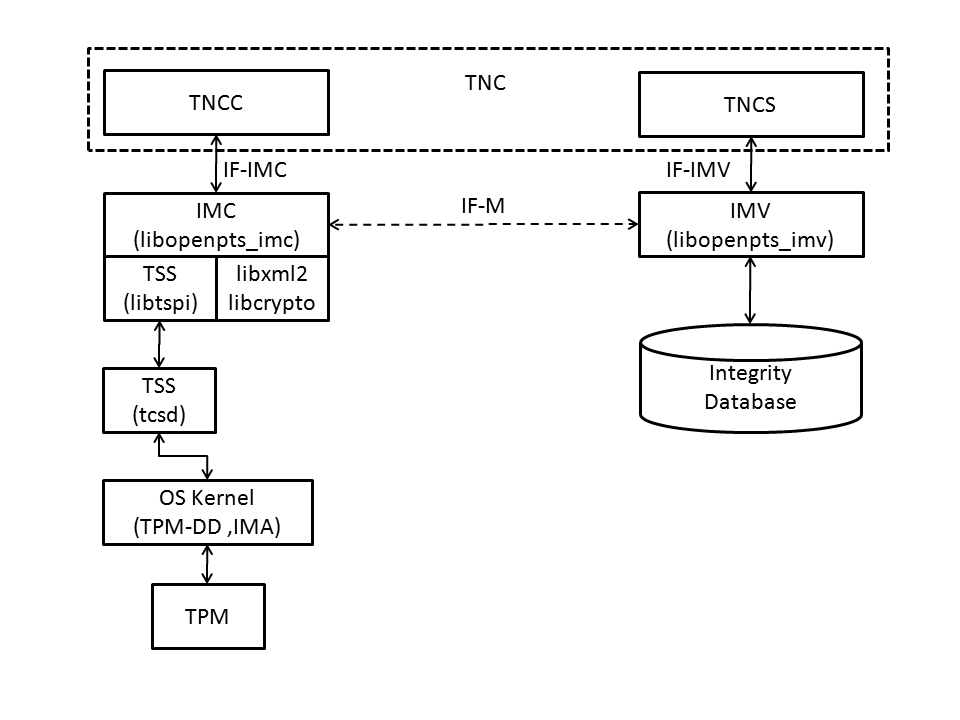
\includegraphics[width=15cm]{OpenPTS_fig_tnc.png}
  \end{center}
  \caption{TNC mode}
  \label{fig:openptstnc}
\end{figure}

\clearpage 

\subsection{Standalone}

OpenPTS also support standalone use. 
In this case, ptscd daemon is running on the target platform as a collector service. 
Remote verifier uses openpts command to attest the remote target.
The ptscd daemon and openpts command use IF-M protocol directly.
If network is not trusted, the message must be pass through secure tunnel. e.g. SSH, SSL/TLS.
 

\begin{figure}[b!p]
  \begin{center}
    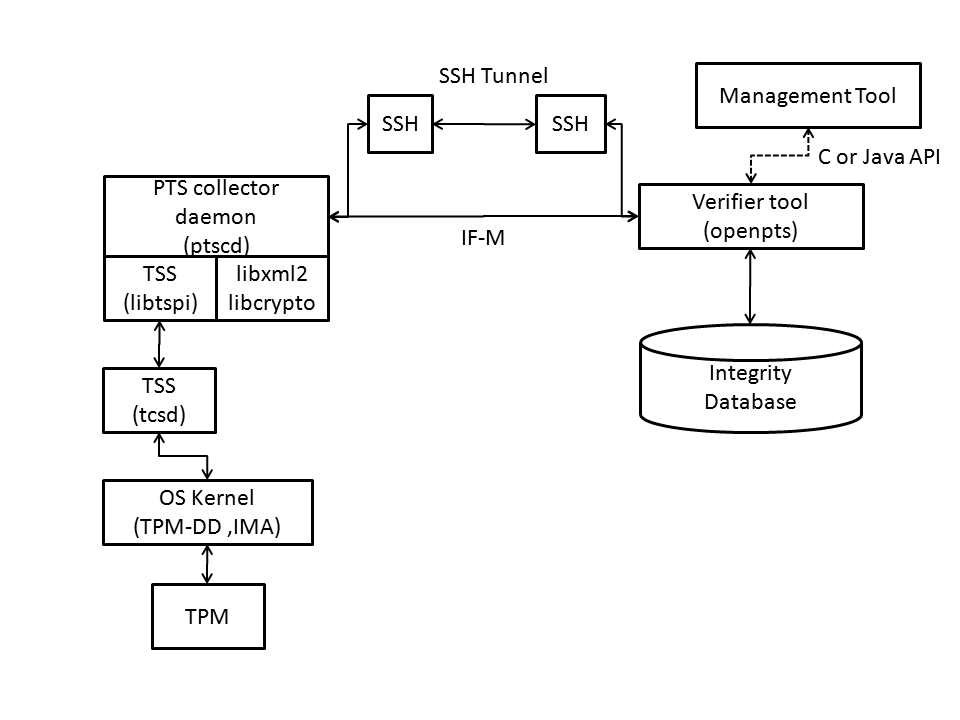
\includegraphics[width=15cm]{OpenPTS_fig_standalone.png}
  \end{center}
  \caption{Standalone mode}
  \label{tncfig} 
\end{figure}

\clearpage 


\subsection{Integrity Measurement}

\subsubsection{SRTM and DRTM}

TBD

\subsubsection{Linux-IMA}

TBD

\subsubsection{OpenPTS}

OpenPTS can measure any files requested by verifier.
The trust of this measurement depend on OpenPTS and underlining components.

\subsection{Validation Engine}

OpenPTS uses Finite State Machine (FSM) models to describe the system.
The boot sequences can be represented by FSMs, 
and the integrity measurement activity of Trusted Computing Platform is an event to drive this FSM.
We use two type of FSM, behavior Model and Binary Model.

behavior Model is used to describe generic software behavior and domain-specific security knowledge of TC, 

Binary Model is correspond to actual binary components to validate the measurements. 

The FSM represents a minimal unit of integrity measurement process, 
and works as a parser of the binay eventlog and then generate the properties.
We use a number of FSM to validate the overall system. 
In our implementation, UML2 State Diagram is used to describe the FSM and integrate 
with standard integrity management architecture proposed by Trusted Computing Group.


\subsubsection{FSM Modeling of Transitive Trust Chain}  

A behavior of the system is modeled as a FSM. 
The IML should be generated to reflect the operation of the system, 
Thus the system is automatically verified through the FSM transition which driven by IML.

Figure \ref{fig:fsm} shows the translation flow from a binary integrity measurement (IML) 
into security properties by using proposed FSM. 
The Validation Engine is a processor of this translation, 
and control the flow of IML and properties. 
The FSM1 feeds the initial properties P0 and the IML, and
finds out the event boundary between FSM1 and FSM2 since the IML contains all events both for
FSM1 and FSM2. The FSM1 generate the rest of events as IML’ and new properties P2 for next
FSM. The FSM2 works in the same manner and generate the final properties P2. The Verification
Result is a final decision made by the Policy Decision Point (PDP) based on the Security Properties
and the Validation Policy.

%The description method of FSM, architecture and implication of lifecycle are discussed in the
%following section.


\begin{figure}[b!p]
  \begin{center}
    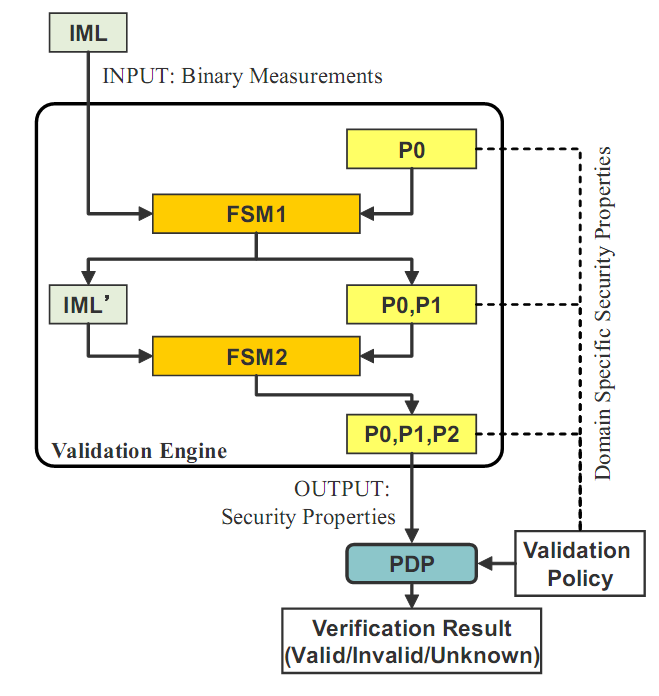
\includegraphics[width=9cm]{OpenPTS_fig1.png}
  \end{center}
  \caption{Translation from binary integrity measurement into security properties}
  \label{fig:fsm} 
\end{figure}



\clearpage 
%%%%%%%%%%%%%%%%%%%%%%%%%%%%%%%%%%%%%%%%%%%%%%%%%%%%%%%%%%%%%%%%%%%%%%%%%%%%%%
%%%%%%%%%%%%%%%%%%%%%%%%%%%%%%%%%%%%%%%%%%%%%%%%%%%%%%%%%%%%%%%%%%%%%%%%%%%%%%
\section{Data Design}
%%%%%%%%%%%%%%%%%%%%%%%%%%%%%%%%%%%%%%%%%%%%%%%%%%%%%%%%%%%%%%%%%%%%%%%%%%%%%%
%%%%%%%%%%%%%%%%%%%%%%%%%%%%%%%%%%%%%%%%%%%%%%%%%%%%%%%%%%%%%%%%%%%%%%%%%%%%%%

\subsection{IF-M Protocol}

PTS IF-M is still DRAFT stage at TCG IWG.


\begin{lstlisting}[label=ifmptnc, caption=IF-M protocol (TNC)]

    TNC
   index       dir          msg
 ---------------------------------------------
     0     IMC -> IMV      (hello)
     1     IMC <- IMV      capability 
     2     IMC -> IMV      capability
 
     3     IMC <- IMV      DH-nonce param req
     4     IMC -> IMV      DH-nonce param res
     5     IMC <- IMV      DH-nonce done
     6     IMC -> IMV      (ack)
 
     7     IMC <- IMV      template RIMM req
     8     IMC -> IMV      RIMM
     9     IMC <- IMV      template IR req
    10     IMC -> IMV      IR

          TNCC <- TNCS/IMV Remidiation
\end{lstlisting}


\begin{lstlisting}[label=ifmptnc, caption=IF-M protocol (standalone)]

             dir        msg
 ---------------------------------------------
         IMC <- IMV   capability 
         IMC -> IMV   capability
 
         IMC <- IMV   DH-nonce param req
         IMC -> IMV   DH-nonce param res
         IMC <- IMV   DH-nonce done
 
         IMC <- IMV   template RIMM req
         IMC -> IMV   RIMM
         IMC <- IMV   template IR req
         IMC -> IMV   IR

         IMC <- IMV   VR
\end{lstlisting}


\subsection{Integrity Report}

TBD


\subsection{Reference Manifest}


TBD


\subsection{UML2 State Diagram}

We use UML2 State Diagram[16] to describe the FSM. The condition of state transition is controlled
by “guard” description. Also, the state has “do” statement to control the property and special
operation by calling the external function.

\ref{umlfig} shows the example diagram and process flow. The IML hold an eventtype and digest
information. The FSM2 represent the domain which has two code regions, and feeds first two events
and generate two additional properties.

\begin{enumerate}
   \item The input properties must contains “P1.integrity = valid” to succeed the CheckProperty state.
       It will be possible to define the dependency between the FSM by using integrity property.
   \item The CODE 0 state check the “P2.digest” property. This is the first code region must be
       measured by the previous FSM, but the reference value is held by this FSM2.
   \item The transition between the CODE 0 and the CODE 1 state is permitted if the first event had
       digest value, 0x04df63ed0fe2856. The behavior is that the CODE 0 measure the CODE 1.
   \item The transition between the CODE 1 and the MEASURE P3 state must be permitted if the
       eventtype of second event was 0x05. The FSM do not care about the digest value in this
       transition since the second event is the code region of next domain measured by the CODE 1.
       This digest value should be checked by next FSM via “P3.digest” property.
   \item Finally, the GenerateProperty state set the property “P2.integrity = valid”.
   \item The third event is not evaluated by the FSM2 and remains to next FSM.
\end{enumerate}

Error transition is abbreviated in this diagram. The transition requirements (= guard expres-
sion) must be set up exclusively to support multiple branches. The FSM must be created for each
PCRs, and will contain number of events correspond to the granularity covered by this. The mani-
fest will contain multiple FSMs, For example, the manifest for PC BIOS contains eight FSMs which
represent of PCR0 to 7 used by BIOS. In addition, the TPM in the lower of figure 2 is an emulator
to calculate the PCR values based on the event processing by FSM. Finally, the Validation Engine
checks the PCR values at the TPM emulator and the values acquired by TPM Quote, and validate
the over all integrity of IML. The description of an event transition by using FSM is easy. But, it
does not fit for subordinated and complicated treatment. We use internal “do” activity to specify
the domain unique and complex function, and keep the simple FSM diagram.

A correspondence of the PTS and XML documents based on the TCG standard and our exten-
sion is shown in \ref{domainfig}. We create the FSM model and domain specific validation functions which
called from the state using “do”. This extension will be integrated with the TCG standard archi-
tecture. The FSM (XML description is generated from UML2 diagram by using XMI)is embedded
in the ReferenceManifest (RM). And the domain specific function is embedded with the PTS.

\begin{figure}[b!p]
  \begin{center}
    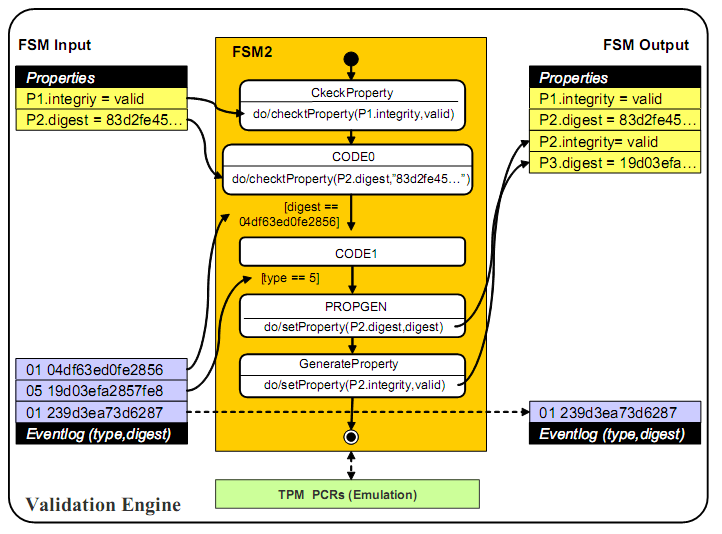
\includegraphics[width=15cm]{OpenPTS_fig2.png}
  \end{center}
  \caption{FSM example by using UML2 state diagram}
  \label{umlfig} 
\end{figure}


\begin{figure}[b!p]
  \begin{center}
    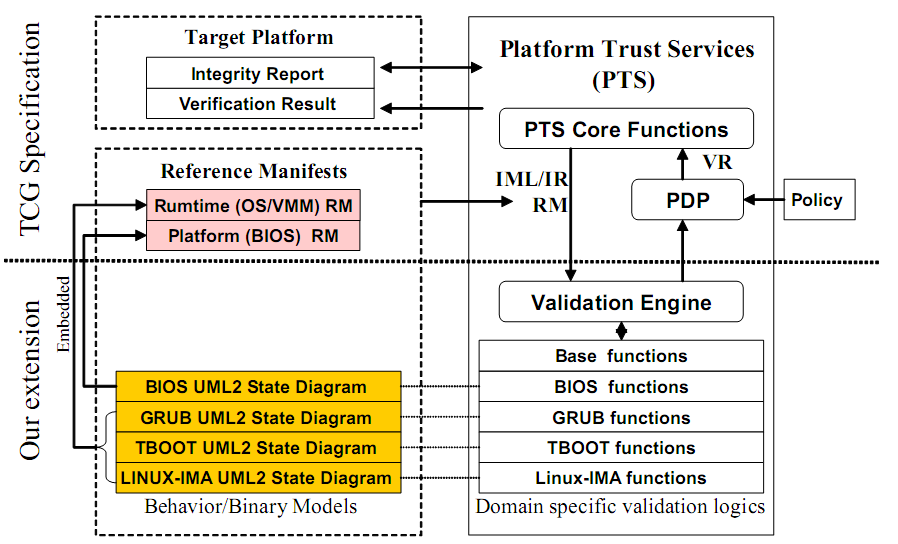
\includegraphics[width=12cm]{OpenPTS_fig3.png}
  \end{center}
  \caption{Domain Specific Architecture/Security Knowledge}
  \label{domainfig} 
\end{figure}


The TCG define the life cycle of the integrity information, called as Integrity Management Model
(IMM) [15]. We want to expand the IMM into software development lifecycle.
\ref{lifecyclefig} shows the life cycle which took in the scheme of our behavior modeling. Under the
present circumstances, we have to create a model for existing software component. But we think

 It is very efficient that the FSM and domain specific validation function in 3 are created in design
stage of software development lifecycle.

     In Software Development Process, we define the Security Properties which a component/domain
has, and such properties will be derived from high-level service requirements. Next, we design the
software to generate the event, and the property could be derived through the validation of events,
and create its Behavior Model by using FSM. The Behavior Model shows general behavior of a
software in the target domain. When software was built up, A Binary Model is created from the
Behavior Model with the actually component hash value to define the concrete transition, and
embedded as part of the Reference Manifest.

     Moreover, The service policy definition is easy since the designed Security Properties and actual
properties translated by FSM from IR and RMs are same.

     When realizing a service corresponded to Trusted Computing, it is impossible for service-
provider to crate a such policy based on the security requirement needed with a service. In this
lifecycle, the property bound up with the measurement at the design phase, and the property is
derived from the measurement at the validation phase. By using proposed scheme, we resolve the
Semantic Gap between binary measurement and security properties.



\begin{figure}[b!p]
  \begin{center}
    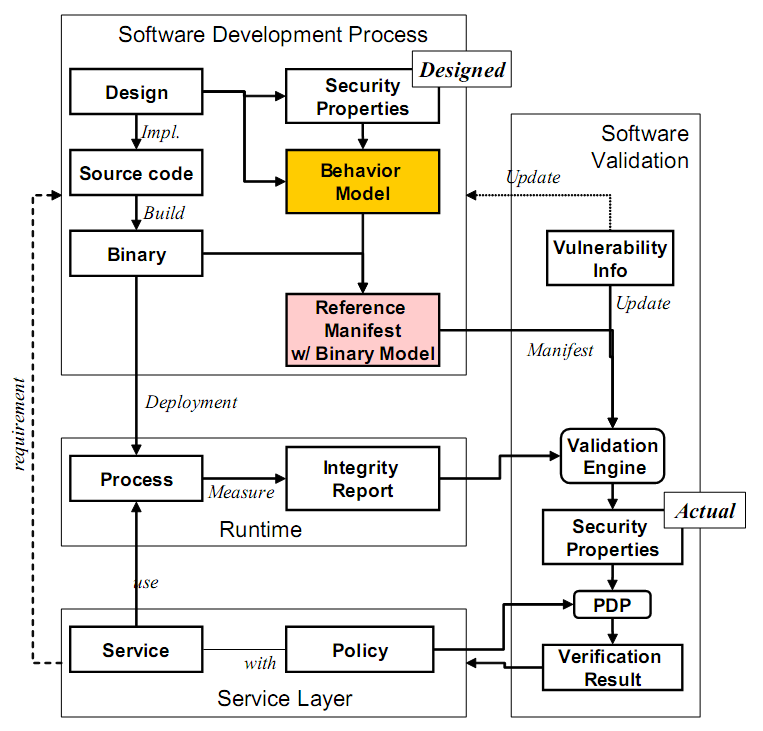
\includegraphics[width=12cm]{OpenPTS_fig4.png}
  \end{center}
  \caption{Software Lifecycle and Integrity Management}
  \label{lifecyclefig} 
\end{figure}



\begin{figure}[b!p]
  \begin{center}
    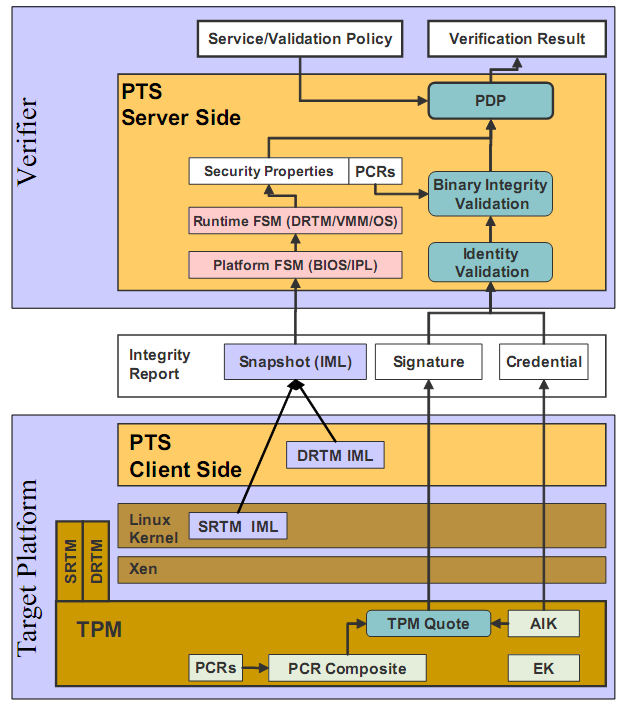
\includegraphics[width=12cm]{OpenPTS_fig5.png}
  \end{center}
  \caption{Manifest and Validation Flow}
  \label{flowfig} 
\end{figure}


\subsubsection{Behavior Models}  

We define four domains, BIOS, IPL, DRTM, and OS. The Behavior Model of PC BIOS is constituted
from eight FSMs to validate the event on PCR0 to PCR7. The TCG PC platform specification [14]
and the BIOS eventlog of actually acquired from existing PCs are referred to created the model. We
found that the trust measurement sequence of BIOS vary widely among each PC vendors. Thus,
our unified BIOS Behavior Model covers all existing BIOS behavior and generate Binary Model
from BIOS eventlog. The FSM for CRTM(PCR0) is explained in Appendix.A.

   For the IPL (Bootloader), the model of GRUB [11] corresponds to PCR4, PCR5 and PCR8
was created. Also we create model for Linux-IMA[2] (PCR10) for OS domain, and tboot[18]
(PCR17,18,19) for DRTM domain. We investigate a behavior of these software and create the
Behavior Model. The Binary Model is created by adding actual hash values taken from binary
code. Appendix. B shows how validation of SRTM by BIOS/GRUB, and DRTM by tboot works
together.



\subsubsection{Do functions}  

The “do” statement used to call external functions which covers complex and special operations.
Table 1 shows the list of functons we implemented for each domains.
   The Validation Engine has TPM emulator to validate the PCR values calculated from the given
IML. To initialize the emulator, we provide two functions, resetSrtmPcr(pcrindex) and resetDrtm-
Pcrpcrindex), these were called by the FSM that use a PCR first. The setProperty (name, value)
and checkProperty (name, value) functions are used to set and verify the property. The above
functions are provided as base functionality.
   For the validation of BIOS eventlog, the addBiosAction() is used for a treatment of Action
Event (evettype = 05h) to generate the BIOS specific properties. The addBiosSpecitficEvent() is
used for a treatment of PC Specific Event (evettype = 06h) to generate the property based on
SMBIOS, NVRAM, and CMOS information in the event.
   For the verify of GRUB eventlog, validateMbr() verifies the MBR of HardDisk which measured

by BIOS. The reason we need the special function to validate the BIOS is, the MBR contains both
code and mutable field, thus the digest may vary for each platform. GRUB-IMA measure the MBR
again and save MBR data as eventdata. The Binary Model contains the digest of MBR which
masked mutable field. Also there are two type of TCG BIOS, one measures 440 bytes, another
measures 446bytes of MBR. The validateMbr() verify the MBR by using this eventdata and the
masked digest. validateEltoritoBootImage() verifies Boot Image which BIOS measures in the case
of startup of an El Torito format CD. Since two kinds of measure exist, one measures the first
512Bytes, another measures 2048Bytes.
    The Model of Linux-IMA uses two functions, the validateImaAggrigate() validate the boot
aggregate event, the validateImaMeasurement() validate the file measured by Linux-IMA with
external Integrity Information Database (IIDB). The Model of tboot uses four functions to validate
the eventlog. It validate the Policy used by tboot and VMM/DOM0 measurement. 


\subsubsection{Supported Model} 


\begin{table}
\caption{BIOS Behavior Models}
\label{table:biosmodel}
\begin{center}
\begin{tabular}{|l|l|}
	\hline
	Model & Description  \\
	\hline 	\hline
	bios\_pcr0.uml &  Static RTM \\
	\hline
	bios\_pcr1.uml &   \\
	\hline
	bios\_pcr2.uml &   \\
	\hline
	bios\_pcr3.uml &   \\
	\hline
	bios\_pcr4.uml &  IPL \\
	\hline
	bios\_pcr5.uml &  IPL config \\
	\hline
	bios\_pcr6.uml &   \\
	\hline
	bios\_pcr7.uml &   \\
	\hline
\end{tabular}
\end{center}
\end{table}


\begin{table}
\caption{IPL and OS Behavior Models}
\label{table:osmodel}
\begin{center}
\begin{tabular}{|l|l|}
	\hline
	Model & Description  \\
	\hline 	\hline
	grub\_pcr4.uml &  Grub stage 1, 1.5, 2 \\
	\hline
	grub\_pcr5.uml &  Grub config \\
	\hline
	grub\_pcr8.uml &  OS measurment by Grub \\
	\hline
	ima\_pcr10.uml &  Linux-IMA \\
	\hline
	ima-ng\_pcr10.uml &  Linux-IMA NG \\
	\hline
	tboot\_pcr17.uml & tboot (DRTM), SINIT  \\
	\hline
	tboot\_pcr18.uml & tboot (DRTM)  \\
	\hline
	tboot\_pcr19.uml & tboot (DRTM)  \\
	\hline
\end{tabular}
\end{center}
\end{table}


\subsubsection{Security Properties} 

Although the properties finally obtained through a validation are drawn from requirement, we
need many interim properties, such property is used as a register of the success or failure state of
FSM, and an exchange of the data between FSMs. We use a property to validate Transitive Trust
Chain. When a validation by FSM come up to final state, it set a corresponding integrity property
to “valid”. And the FSM must check all the integrity properties generated by underling FSM to
validate the dependency of FSMs. We can select the PCR for TPM Quote operation but sufficiency
of this selection is not formulated. By using interim properties, we easily know and describe the
dependency between PCRs, and FSMs too).

Another reason an exchange of a property between FSMs is, the measurement of a component
being dependent on the loader side design. Therefore, the IML is parsed by loader side FSM which
understands how the IML was generated, and it set the measurement (digest value) to the property
for successive FSM which know the reference digest value. We need to use common properties to
interlock the FSMs. Current list of integrity property is defined in table 2.

\subsection{Validation Policy} 

TBD 


\subsubsection{SCAP} 


TBD



\clearpage 
%%%%%%%%%%%%%%%%%%%%%%%%%%%%%%%%%%%%%%%%%%%%%%%%%%%%%%%%%%%%%%%%%%%%%%%%%%%%%%
%%%%%%%%%%%%%%%%%%%%%%%%%%%%%%%%%%%%%%%%%%%%%%%%%%%%%%%%%%%%%%%%%%%%%%%%%%%%%%
\section{Component Design}
%%%%%%%%%%%%%%%%%%%%%%%%%%%%%%%%%%%%%%%%%%%%%%%%%%%%%%%%%%%%%%%%%%%%%%%%%%%%%%
%%%%%%%%%%%%%%%%%%%%%%%%%%%%%%%%%%%%%%%%%%%%%%%%%%%%%%%%%%%%%%%%%%%%%%%%%%%%%%

\subsection{Required Components}

\begin{table}
\caption{Linux}
\label{table:timeline}
\begin{center}
\begin{tabular}{|l|l|l|}
	\hline
	Components & RPM package name & DEB package name \\
	\hline 	\hline
	libtspi.so   & trousers & trousers \\ \hline
	libxml2.so   & libxml2  & libxml2  \\ \hline
	libcrypto.so & openssl  & openssl  \\ \hline
	libuuid.so   & libuuid  & libuuid  \\ \hline
\end{tabular}
\end{center}
\end{table}


\subsection{Binaries}


\subsubsection{libopenpts\_imv and libopenpts\_imc}

TBD


\subsubsection{ptscd}

TBD

\subsubsection{openpts}

TBD

\subsection{Configurations}

TBD

TBD

\subsubsection{/usr/share/openpts}

FSM Models

\subsubsection{/etc/openpts.conf}

TBD
 
\subsubsection{/var/lib/openpts}

TBD

\subsection{Integrity Database}

TBD

\subsubsection{IIDB (MySQL,PostgreSQL)}

\begin{figure}[b!p]
  \begin{center}
    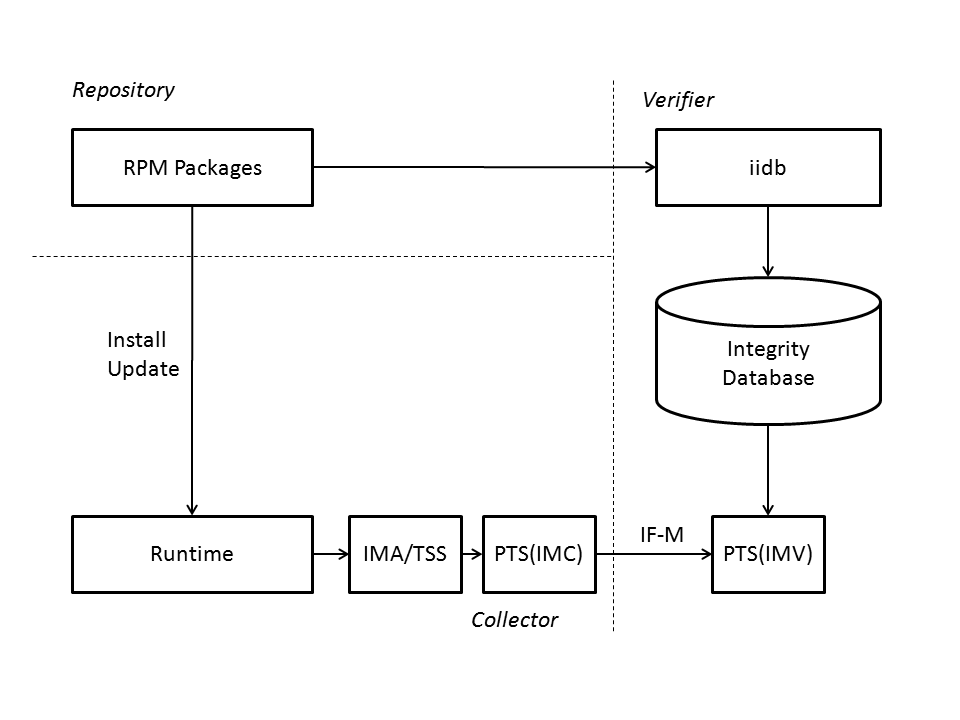
\includegraphics[width=12cm]{OpenPTS_fig_iidb.png}
  \end{center}
  \caption{IIDB}
  \label{fig:iidb} 
\end{figure}


\clearpage 
%%%%%%%%%%%%%%%%%%%%%%%%%%%%%%%%%%%%%%%%%%%%%%%%%%%%%%%%%%%%%%%%%%%%%%%%%%%%%%
\subsubsection{AIDE (Linux)}
%%%%%%%%%%%%%%%%%%%%%%%%%%%%%%%%%%%%%%%%%%%%%%%%%%%%%%%%%%%%%%%%%%%%%%%%%%%%%%

AIDE (Advanced Intrusion Detection Environment)\cite{aide} is a free replacement for Tripwire. It does the same things as the semi-free Tripwire and more.

OpenPTS can use an integrity database created by AIDE.


\begin{verbatim}

Sample AIDE policy work with IMA

/etc/aide.conf
---
@@define DBDIR /var/lib/aide
@@define LOGDIR /var/log/aide
database=file:@@{DBDIR}/aide.db.gz
database_out=@@{DBDIR}/aide.db.new.gz
gzip_dout=yes
report_url=file:@@{LOGDIR}/aide.log

IMA = p+u+g+acl+xattrs+sha1+sha256+sha512

/bin IMA
/sbin IMA
/lib IMA
/usr/bin IMA
/usr/sbin IMA
/usr/lib IMA
/etc IMA
/boot IMA
---

extract initrd for AIDE

mkdir /boot/initramfs
cd /boot/initramfs
zcat ../initramfs-2.6.xx.x.img | cpio -id


$ aide --init


$ aide --check

$ aide --update

mv /var/lib/aide/aide.db.new.gz /var/lib/aide/aide.db.gz


AIDE commands         
    --init, -i                          initialize database
    --check, -C                         check the database for inconsistencies
    --update, -u                        check and update database
    --compare                           compares two database
    --config-check, -D                  Stop after reading the config file
    --config=configfile                 set config file


\end{verbatim}


\begin{verbatim}

openpts --init -h 192.168.0.1 -p 5570 --db=aide

get RM and aidb.db from target
stored in

/var/lib/openpts/target/[UUID]/platform_rm.xml
/var/lib/openpts/target/[UUID]/runtime_rm.xml
/var/lib/openpts/target/[UUID]/aide.db.gz



openpts --check -h 192.168.0.1 -p 5570 --db=aide





\end{verbatim}




% Ubuntu
% sudo apt-get install aide
%  /etc/aide/aide.conf.d/
%
% aideinit   (instead of  aide --init)
%
%

\begin{figure}[b!p]
  \begin{center}
    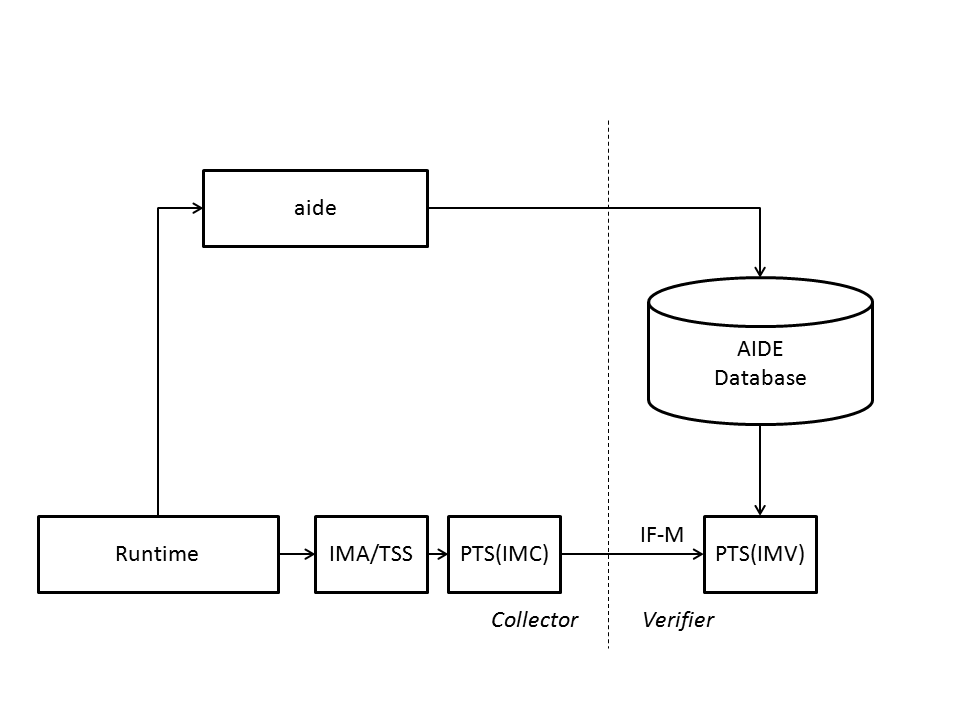
\includegraphics[width=12cm]{OpenPTS_fig_aide.png}
  \end{center}
  \caption{AIDE}
  \label{fig:aide} 
\end{figure}


TBD


\clearpage 
%%%%%%%%%%%%%%%%%%%%%%%%%%%%%%%%%%%%%%%%%%%%%%%%%%%%%%%%%%%%%%%%%%%%%%%%%%%%%%
\subsection{Logging}
%%%%%%%%%%%%%%%%%%%%%%%%%%%%%%%%%%%%%%%%%%%%%%%%%%%%%%%%%%%%%%%%%%%%%%%%%%%%%%

TBD

\subsubsection{syslog}

TBD 

\subsubsection{Debug}

TBD

%%%%%%%%%%%%%%%%%%%%%%%%%%%%%%%%%%%%%%%%%%%%%%%%%%%%%%%%%%%%%%%%%%%%%%%%%%%%%%
%%%%%%%%%%%%%%%%%%%%%%%%%%%%%%%%%%%%%%%%%%%%%%%%%%%%%%%%%%%%%%%%%%%%%%%%%%%%%%
\section{Commands}
%%%%%%%%%%%%%%%%%%%%%%%%%%%%%%%%%%%%%%%%%%%%%%%%%%%%%%%%%%%%%%%%%%%%%%%%%%%%%%
%%%%%%%%%%%%%%%%%%%%%%%%%%%%%%%%%%%%%%%%%%%%%%%%%%%%%%%%%%%%%%%%%%%%%%%%%%%%%%

OpenPTS provides several commands. 
For detailed information, please refer to User's Guide.


%%%%%%%%%%%%%%%%%%%%%%%%%%%%%%%%%%%%%%%%%%%%%%%%%%%%%%%%%%%%%%%%%%%%%%%%%%%%%%
\section{Testing}
%%%%%%%%%%%%%%%%%%%%%%%%%%%%%%%%%%%%%%%%%%%%%%%%%%%%%%%%%%%%%%%%%%%%%%%%%%%%%%

\subsubsection{Unit Testing}

OpenPTS uses unit test tool, 'check'.

\subsubsection{Static Analysis}

Use static analysis tools to find bugs.

\subsubsection{Dynamic Analysis}

Use 'vlagrind' to check the memory leak. 

\subsubsection{Fuzzer}

Use fuzzing test for the IF-M protocol.


\clearpage 
%%%%%%%%%%%%%%%%%%%%%%%%%%%%%%%%%%%%%%%%%%%%%%%%%%%%%%%%%%%%%%%%%%%%%%%%%%%%%%
\section{Requirements Matrix}
%%%%%%%%%%%%%%%%%%%%%%%%%%%%%%%%%%%%%%%%%%%%%%%%%%%%%%%%%%%%%%%%%%%%%%%%%%%%%%


\begin{table}
\caption{Requirements Matrix}
\label{table:reqmatrix}
\begin{center}
\begin{tabular}{|l|l|l|l|}
	\hline
	Requirements & 0.1.X & 0.2.X & 0.3.X \\
	\hline 	\hline
	Java           & Y  & Y(0.2.2)  &   \\ \hline
	C              &    & Y         &   \\ \hline
	IWG XML schema & Y  & Y         &   \\ \hline
	FSM models     & Y  & Y(update) &   \\ \hline
    SRTM           & Y  & Y(update) &   \\ \hline
    DRTM           &    & Y(0.2.3)  &   \\ \hline
	IF-M           &    & Y         &   \\ \hline
	IMA            & Y  & Y(update) &   \\ \hline
\end{tabular}
\end{center}
\end{table}


\clearpage 


\addcontentsline{toc}{section}{References}

\begin{thebibliography}{9}


% http://www.trustedcomputinggroup.org/developers/infrastructure

\bibitem{tcgarch}
  TCG Architecture Overview, Version 1.4
  %\url{http://www.trustedcomputinggroup.org/resources/tcg_architecture_overview_version_14}

\bibitem{core_integrity_schema}
  Infrastructure Work Group Core Integrity Schema Specification, Version 1.0.1
  %\url{http://www.trustedcomputinggroup.org/resources/infrastructure_work_group_core_integrity_schema_specification_version_101}

\bibitem{simple_object_schema}
  Infrastructure Work Group Simple Object Schema Specification, Version 1.0
  %\url{http://www.trustedcomputinggroup.org/resources/infrastructure_work_group_simple_object_schema_specification_version_10}

\bibitem{rm_schema}
  Infrastructure Work Group Reference Manifest (RM) Schema Specification, Version 1.0
  %\url{http://www.trustedcomputinggroup.org/resources/infrastructure_work_group_reference_manifest_rm_schema_specification_version_10}

\bibitem{integrity_report_schema}
  Infrastructure Work Group Integrity Report Schema Specification, Version 1.0
  %\url{http://www.trustedcomputinggroup.org/resources/infrastructure_work_group_integrity_report_schema_specification_version_10}

\bibitem{verification_result_schema}
  Infrastructure Work Group Verification Result Schema Specification, Version 1.0 
  %\url{http://www.trustedcomputinggroup.org/resources/infrastructure_work_group_verification_result_schema_specification_version_10}

\bibitem{qualities_schema}
  Infrastructure Work Group Security Qualities Schema Specification Version 1.1, Revision 7.0
  %\url{http://www.trustedcomputinggroup.org/resources/infrastructure_work_group_security_qualities_schema_specification}


\bibitem{pts}
  Infrastructure Work Group Platform Trust Services Interface Specification, Version 1.0
  %\url{http://www.trustedcomputinggroup.org/resources/infrastructure_work_group_platform_trust_services_interface_specification_version_10}

\bibitem{ifpts}
  Infrastructure Work Group Platform Trust Services Interface Specification (IF-PTS) Version 1.0
  %\url{http://www.trustedcomputinggroup.org/resources/infrastructure_work_group_platform_trust_services_interface_specification_ifpts_version_10}

\bibitem{ifmpts}
  IF-M PTS (DRAFT)

\bibitem{tncarch}
  TNC Architecture for Interoperability Version 1.4, Revision 4, 
  %\url{http://www.trustedcomputinggroup.org/resources/tnc_architecture_for_interoperability_specification}

\bibitem{ifmtlv}
  TNC IF-M: TLV Binding Version 1.0, Revision 37, 
  %\url{http://www.trustedcomputinggroup.org/resources/tnc_ifm_tlv_binding_specification}

\bibitem{ifimc}
  TNC IF-IMC Specification, Version 1.2
  %\url{http://www.trustedcomputinggroup.org/resources/tnc_ifimc_specification}

\bibitem{ifimv}
  TNC IF-IMV Specification, Version 1.2, Revision 8
  %\url{http://www.trustedcomputinggroup.org/resources/tnc_ifimv_specification}

\bibitem{aide}
  AIDE - Advanced Intrusion Detection Environment
  %\url{http://www.cs.tut.fi/~rammer/aide.html}

\end{thebibliography}


\clearpage 
%%%%%%%%%%%%%%%%%%%%%%%%%%%%%%%%%%%%%%%%%%%%%%%%%%%%%%%%%%%%%%%%%%%%%%%%%%%%%%
\appendix
\section{FSM Models}
%%%%%%%%%%%%%%%%%%%%%%%%%%%%%%%%%%%%%%%%%%%%%%%%%%%%%%%%%%%%%%%%%%%%%%%%%%%%%%

\begin{figure}[h]
  \begin{center}
    \includegraphics[width=16cm]{../models/bios_pcr0.png}
  \end{center}
  \caption{BIOS PCR0}
  \label{fig:fsm:biospcr0} 
\end{figure}

\begin{figure}[h]
  \begin{center}
    \includegraphics[width=18cm]{../models/bios_pcr1.png}
  \end{center}
  \caption{BIOS PCR1}
  \label{fig:fsm:biospcr1} 
\end{figure}

\begin{figure}[h]
  \begin{center}
    \includegraphics[width=17cm]{../models/bios_pcr2.png}
  \end{center}
  \caption{BIOS PCR2}
  \label{fig:fsm:biospcr2} 
\end{figure}

\begin{figure}[h]
  \begin{center}
    \includegraphics[width=5cm]{../models/bios_pcr3.png}
  \end{center}
  \caption{BIOS PCR3}
  \label{fig:fsm:biospcr3} 
\end{figure}

\begin{figure}[h]
  \begin{center}
    \includegraphics[width=9cm]{../models/bios_pcr4.png}
  \end{center}
  \caption{BIOS PCR4}
  \label{fig:fsm:biospcr4} 
\end{figure}

\begin{figure}[h]
  \begin{center}
    \includegraphics[width=6cm]{../models/bios_pcr5.png}
  \end{center}
  \caption{BIOS PCR5}
  \label{fig:fsm:biospcr5} 
\end{figure}

\begin{figure}[h]
  \begin{center}
    \includegraphics[width=6cm]{../models/bios_pcr6.png}
  \end{center}
  \caption{BIOS PCR6}
  \label{fig:fsm:biospcr6} 
\end{figure}

\begin{figure}[h]
  \begin{center}
    \includegraphics[width=5cm]{../models/bios_pcr7.png}
  \end{center}
  \caption{BIOS PCR7}
  \label{fig:fsm:biospcr7} 
\end{figure}

\begin{figure}[h]
  \begin{center}
    \includegraphics[width=18cm]{../models/grub_pcr4.png}
  \end{center}
  \caption{GRUB PCR4}
  \label{fig:fsm:grubpcr4} 
\end{figure}

\begin{figure}[h]
  \begin{center}
    \includegraphics[width=15cm]{../models/grub_pcr5.png}
  \end{center}
  \caption{GRUB PCR5}
  \label{fig:fsm:grubpcr5} 
\end{figure}

\begin{figure}[h]
  \begin{center}
    \includegraphics[width=10cm]{../models/grub_pcr8.png}
  \end{center}
  \caption{GRUB PCR8}
  \label{fig:fsm:grubpcr8} 
\end{figure}

\end{document}
